\documentclass[../main.tex]{subfiles}

\begin{document}

\section{Lectures 5 and 6}

\subsection{Quiz Lecture 5}
\pp{1}
Floating Point Cancellation
For which of the following reasons is cancellation in floating-point computation usually bad?

Choice*
The digits lost are the least significant.
The digits lost are the most significant.
The result is usually not exactly representable.
Subsequent operations are likely to underflow or overflow.

\begin{solution}
    The digits lost during catastrophic cancellation are the most significant ones (ie the left most ones). Since we're losing digits in the resultant answer, our answer is often exactly representable (remember that we have about $-\log(2^{-52}) \approx 16 = -\log(10^{-16})$ digits of relative accuracy).
\end{solution}

\pp{2}
Cancellation and Rounding
Which of the following statements is true regarding the relationship between rounding and cancellation?

Choice*
In computation that is done with exact (not rounded) values, cancellation cannot occur.
Catastrophic cancellation occurs when cancellation amplifies rounding errors in the input.
Subtracting two rounded numbers will always amplify the error.
Cancellation from subtracting two rounded inputs of similar magnitude and sign can be reduced by first converting the rounded inputs to higher precision.
\begin{solution}
    Even with exact values, we can find that leading digits are chopped off, if the two numbers agree to a high number of decimal places. Yes, catastrophic cancellation is the phenemonon that takes places when we subtract so much from a number that whatever is shifted upwards to replace the nullified digits is inaccurate, rounding error. This does not mean that subtracting any two numbers will always amplify rounding error, however. Even if you convert numbers to higher precision, this will not change the fact that cancellation will take place -- several initial numbers will still match; it will reduce the chances of catastrophic cancellation taking place, however.
\end{solution}

\pp{3}
Cancellation and Relative Error
Suppose a and b are stored in single precision and agree to four decimal digits. Assume a is known to seven decimal digits and b is known to five decimal digits.

Let c=b−a.

Accounting only for cancellation error, how many decimal digits of accuracy are in c?


How many decimal digits are in c after accounting for the relative error in a and b?

\begin{solution}
    In single precision, we have $-\log(2^{-22}) \approx 7$ digits of accuracy. Thus, $a$ and $b$ are (ignoring their relative accuracies initially) known really to $7$ digits, so that if subtract them and nullify their first $4$ digist, then there are only $3$ digits that remain. If we account for relative error in the subtraction, however, then there are only $\min{7-4, 5-4} = 1$ digits that are accurate.
\end{solution}

\pp{4}
Changing the RHS
You just solved a linear system Ax=b. Unfortunately, the RHS b that you solved it with was wrong.

Worried, you compute
‖Δb‖‖b‖≈10−12.
The condition number of your matrix is about 10000.

What could your worst-case relative error in the solution x be due to your use of the wrong RHS?

\begin{solution}
    Just multiply condition number by relative input error.
\end{solution}

\pp{5}
Distance to Singularity
Which of the following is a good indicator that a matrix is nearly (as measured by the matrix norm) singular?

Choice*
Its norm is small.
Its determinant is small.
Its condition number is large.
Its norm is large.

\begin{solution}
    $k(\gamma A) = k(A)$. That is, no scaling of a matrix can change its condition number; all the other quantities can change very much, however.
\end{solution}

\pp{6}

What is the $2$ norm of a diagonal matrix:

\begin{solution}
    It is the maximum of teh diagonal entries. The condition number is the ratio of the maximum diagonal entry in absolute value to the minimum one in absolute value.
\end{solution}


\subsection{Quiz for Lecture 6}
Relative Residual
Consider a matrix $A=\begin{bmatrix} −9 & -5 \\ 8 & 3 \end{bmatrix}$ and right-hand side vector b=[3−2]. Using the infinity norm, calculate the relative residual if elements of the solution vector xˆ are rounded to one significant digit. Include at least three significant digits in your answer.

\begin{solution}
    $\norm{A} = 14$. Let $\hat{x} = \inv{A}b = \begin{bmatrix}
        -0.08 \\ 0.5
    \end{bmatrix}$ if you round to $1$ digit. Then $r = A\hat{x} - b = \begin{bmatrix}
        -0.22 \\
        0.14 \\
    \end{bmatrix}$

    Meaning that $\norm{r} = 0.22$. And $\norm{x} = 0.5$

    \[
        \frac{\norm{r}}{\norm{x}\norm{A}} = \frac{0.22}{0.5 * 15}
    \]

    which is correct.
\end{solution}

\pp{2}

A stupid definition question.

\pp{3}
Gaussian Elimination
In the following questions, consider Gaussian elimination with the prescribed pivoting strategy to generate the lower (L) and upper (U) triangular factors for the following matrix,

\[
    A = \begin{bmatrix}
       2 & 1 & 3 \\
       2 & 4 & 8 \\
       4 & -7 & 4 \\
    \end{bmatrix}
\]

Know that with pivoting, we must first swap rows $1$ and $3$ and then perform gaussian elimination.


\pp{4}
Existence of LU Decomposition with no Pivoting
For which of the following matrices does a LU factorization without pivoting not exist?

\begin{solution}
    I have

\begin{center}
    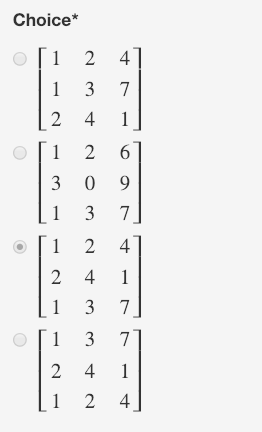
\includegraphics[width=\textwidth,height=\textheight,keepaspectratio]{lecture6_quiz_q4}

    Sufficient Condition: If a pivot is $0$ (assuming that we don't pivot the matrix when performing gaussian elimination), then the matrix will fail to provide an LU factorization.
\end{center}
\end{solution}

\pp{5}
Just apply

\[
    \text{rel error} \leq k(A) \frac{\norm{r}}{\norm{A}\norm{x}} 
\]

\pp{6}
\begin{center}
    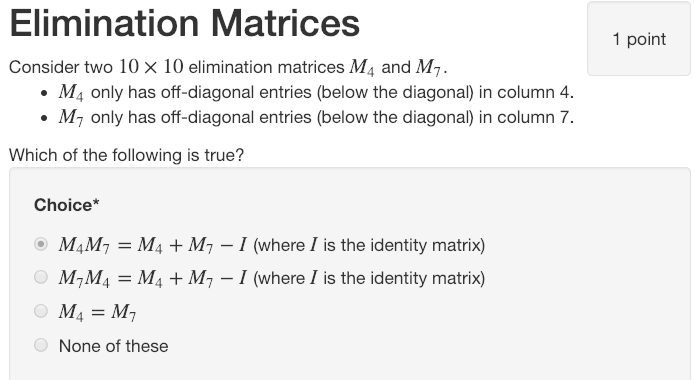
\includegraphics[width=\textwidth,height=\textheight,keepaspectratio]{lecture6_quiz_q6}

    Note that elimination matrices must progress from left to right, meaning that elimination matrices $M_1$ and $M_2$ must be such that the off diagonal entry of $M_1$ is left of the off diagonal entry of $M_2$, if we want $M_1 M_2$ to merge.
\end{center}


\breathe \\

The following is the definition of the residual.
\begin{center}
    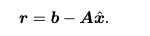
\includegraphics[width=\textwidth,height=\textheight,keepaspectratio]{lec6_resid}
\end{center}

\begin{remark}
    The residual itself does not reveal much. Suppose we calculate $r = b - Ax$. Now solve for $kAx = kb$ and the residual required to solve that is $k$ times as great. This is why we define the relative residual:

    \[
        \frac{\norm{r}}{\norm{A} \cdot \norm{\hat{x}}}
    \]
\end{remark}

We can obtain a bound on the relative forward error required to solve $Ax = b$ in terms of $r$.
\begin{center}
    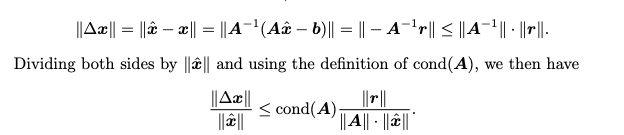
\includegraphics[width=\textwidth,height=\textheight,keepaspectratio]{lec6_residBound}
\end{center}

\begin{remark}
    This bound tells us that if the residual is small and the matrix and well conditioned, then the relative error is low.
\end{remark}

\begin{center}
    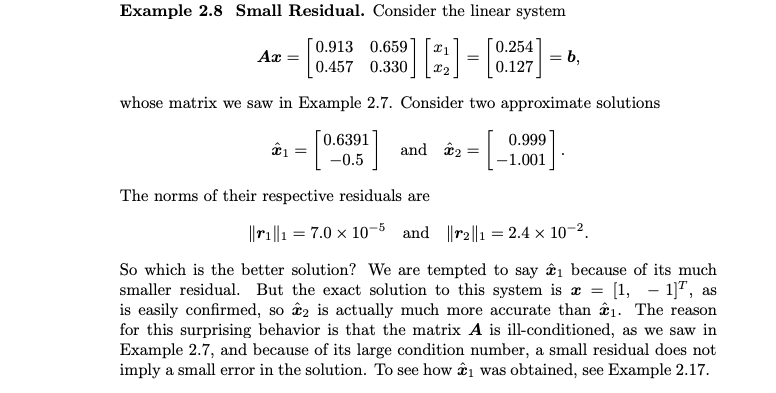
\includegraphics[width=\textwidth,height=\textheight,keepaspectratio]{lec6_residExample}
\end{center}

\begin{center}
    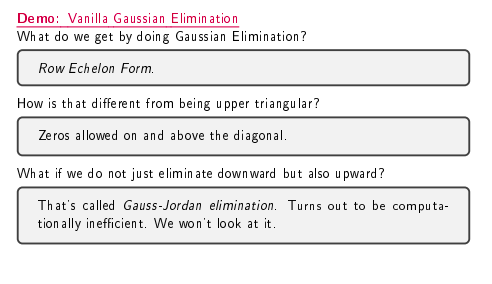
\includegraphics[width=\textwidth,height=\textheight,keepaspectratio]{lec6_rowE}
\end{center}

\begin{remark}
    Also note that a matrix is in row echelon form if the first non-zero entry of each row (what was the pivot during gaussian elimination) is to the right of the first non-zero entry of any preceding row; moreover, entries in rows above the pivot (but in the same column) must be $0$.
\end{remark}

\begin{center}
    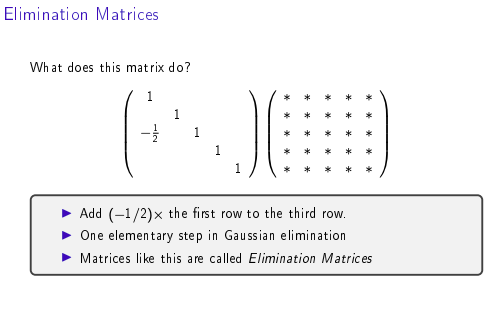
\includegraphics[width=\textwidth,height=\textheight,keepaspectratio]{lec6_elimM}
\end{center}

\begin{remark}
    If we add $k$ to the identity matrix at entry $i,j$, and left multiply the resultant
    matrix $C$ by some matrix of interest $A$, then the result is to take the $j$ th row of $A$
    multiply it by $k$ and then add it to $i$. We can undo this process by using the same
    matrix but, in place of $k$, using $-k$. This second matrix is the inverse to the elimination matrix $C$.
\end{remark}

\begin{center}
    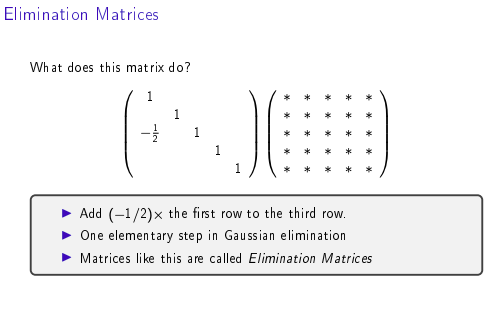
\includegraphics[width=\textwidth,height=\textheight,keepaspectratio]{lec6_elimM}
\end{center}


\begin{remark}
    Suppose that we multiply $A$ by an elimination matrix $M_1$, then by $M_2$ up to $M_l$,
    where $M_l$ is the last matrix required to turn $A$ into Row Echelon Form.
    Eventually, we will have 

    \[
        (M_l \dots M_1)A = U \implies A =  \inv{(M_l \dots M_1)}U
    \]

    At first glance, this is okay, because it turns out that left multiplication of an elimination matrix $X$ by $Y$ such that $X$ has a non-zero off diagonal at column $i$ and $Y$ has a non-zero off diagonal at column $j$ where $i < j$ results in an elimination matrix that just merges $X$ and $Y$ \footnote{Note that merging also takes place if we multiply two elimination matrices that have their off diagonal non-zero entry in the same column as each other.}

    For whatever reason, pivoting foils this attempt:

    \begin{center}
        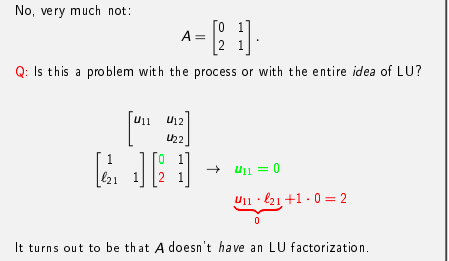
\includegraphics[width=\textwidth,height=\textheight,keepaspectratio]{lec6_pivotfail}
    \end{center}

    The solution is to repeatedly apply permutations to $A$ (in the form
    of permutation matrices) so that the pivot is the largest element
    in terms of absolute value in its column.

    Thus, we now have

    \[
        (M_lP_l \dots M_1P_1)A = U \implies A = \inv{(M_lP_l \dots M_1P_1)}U
    \]

    However, what should be $L$ above is not always left triangular. It can be shown that a factorization of $\inv{(M_lP_l \dots M_1P_1)}$ does, however, give us a lower triangular system.
\begin{center}
    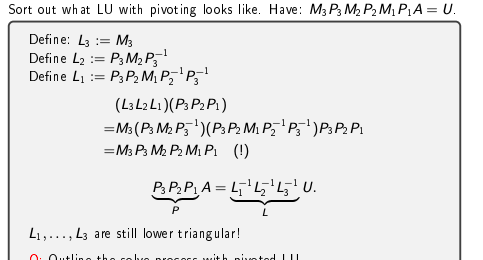
\includegraphics[width=\textwidth,height=\textheight,keepaspectratio]{lec6_pivotres}
\end{center}
\end{remark}

\begin{center}
    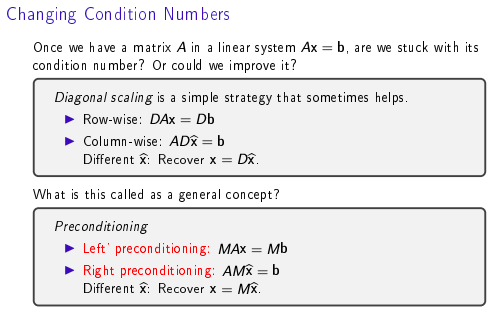
\includegraphics[width=\textwidth,height=\textheight,keepaspectratio]{lec6_precond}
\end{center}
\begin{remark}
    Suppose that $D$ above satisfies $k(D) \approx 1$. Then

    \[
        k(DA) = \norm{DA}\norm{\inv{(DA)}} \leq \norm{D}\norm{A}\norm{\inv{A}}\norm{\inv{D}} \leq k(A)
    \]

    so that the condition number of $K(DA)$ is no greater than the condition number of $A$.

    Assuming that $D$ is invertible, then the set of $x$ satisfying
    $Ax = b$ is precisely the set of $x$ satisfying $Ax = b$. Left multiplication
    by $D$ of $A$ is called, understandably, left preconditioning and scales
    $A$ in a row-wise manner; right multiplication by $D$ of $A$ is called right
    preconditioning.
\end{remark}


\begin{remark}
\begin{center}
    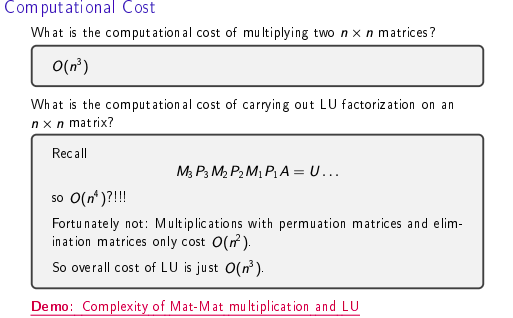
\includegraphics[width=\textwidth,height=\textheight,keepaspectratio]{lec6_compCost}
\end{center}

Multiplication by a permutation matrix is only an $n$ operation, since it involves switching rows. Multiplication by an elimination matrix simply involves scaling one row and mulitplying it by another, and this process is done at most $n$ times for any one elimination matrix (making it $O(n^2)$ as well). Since these transformations are applied at most $n$ times, the process of getting a matrix into $LU$ form is only $O(n^3)$.
\end{remark}

\begin{remark}

\begin{center}
    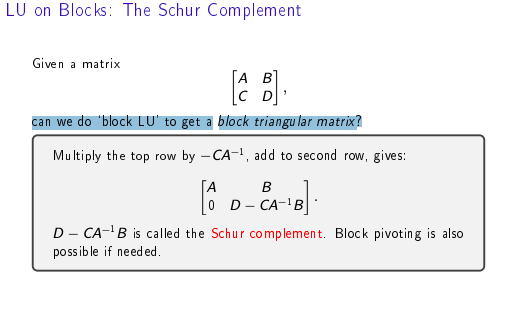
\includegraphics[width=\textwidth,height=\textheight,keepaspectratio]{lec6_luBlocks}
\end{center}

Not sure why this is significant.

\end{remark}


\begin{remark}
    Unresolved
\begin{center}
    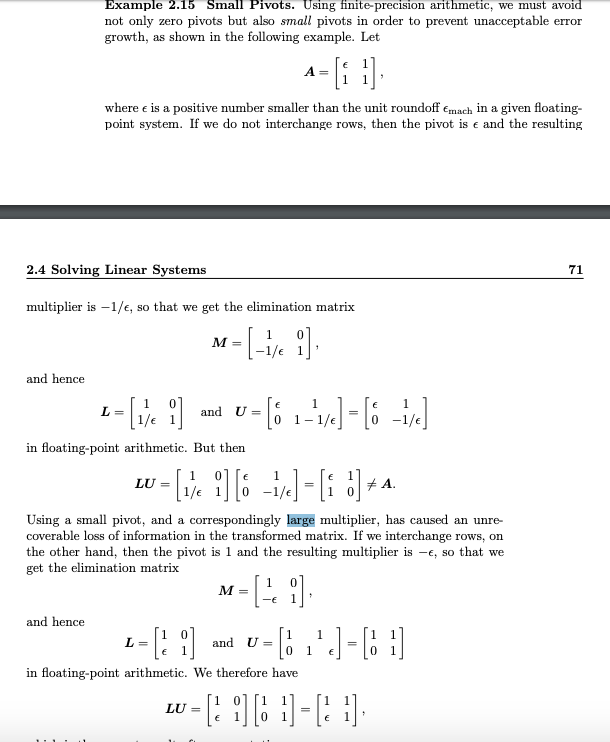
\includegraphics[width=\textwidth,height=\textheight,keepaspectratio]{lec6_smallPivotsBad}
\end{center}
\end{remark}

\begin{remark}
    Notice that if we already have an $LU$ factorization, then computing a rank $1$ update is just an $O(n^2)$ operation.
\begin{center}
    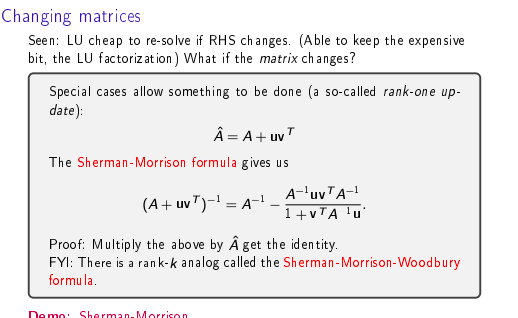
\includegraphics[width=\textwidth,height=\textheight,keepaspectratio]{lec6_shermanMorrison}
\end{center}

For 

\[
    \left( A + uv^T \right)^{-1}b = \inv{A}b - \frac{\left( \inv{A}u \right)v^T\inv{A}b}{1 + v^T\inv{A}u}
\]

And $\inv{A}x$ for any $x$ is an $O(n^2)$ operation. The only other operation in this formula is to compute a dot product.
\end{remark}

\begin{remark}
    \begin{center}
        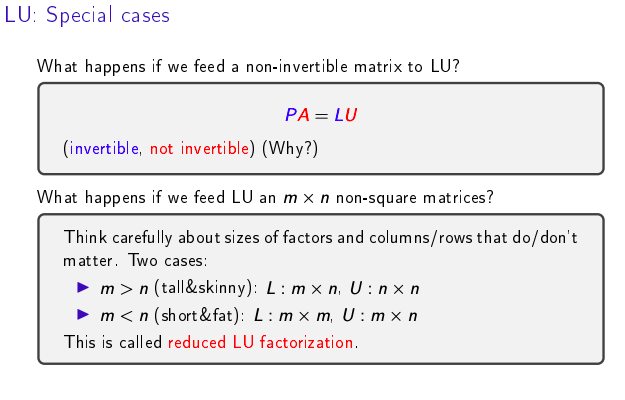
\includegraphics[width=\textwidth,height=\textheight,keepaspectratio]{lecture6_lu_special}
    \end{center}

    A matrix $A$ always admits an LU factorization, even if $A$
    is singular. First, observe that every column of $A$ must contain
    at least one non-zero number -- or else, why would the column
    be part of $A$. Thus, if a pivot entry does not contain a non-zero
    value, we can rotate rows so that the pivot entry does have
    a non-zero value. We then can apply elimination matrices, as needed,
    until all row values in the pivot's column are $0$. 

    The foregoing tells us that there still exists a sequence of
    permutations and elimination matrices that bring $A$ into upper
    triangular form. Since these matrices are each invertible, it follows that $L$ is still invertible. Since $\abs{PA} = 0$, we must have, therefore, $\abs{U} = 0$, which means that $0$ must occupy some diagonal entry of $U$.

    Why? A matrix fails to be invertible iff $0$ is an eigenvalue. $0$ is an eigenvalue iff some entry on the diagonal is $0$, because the eigenvalues of a triangular matrix are precisely its diagonal entries.

    Why are permutation matrices invertible? Group theory promises us that some power of a permutation brings it back to the identity. That is $P^k = I$ for some $I$. Thus $\inv{P} = P^{k-1}$.
\end{remark}

\begin{remark}
    Why can we take an $LU$ decomposition and then reduce it, as shown below?
    \begin{center}
        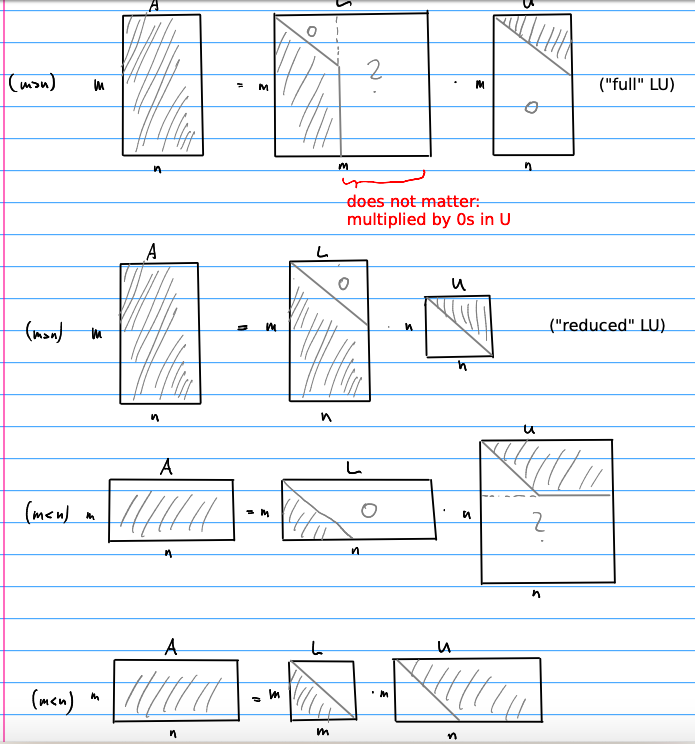
\includegraphics[width=\textwidth,height=\textheight,keepaspectratio]{lecture6_lu_reduced}
    \end{center}

    If $m > n$, applying elimination matrices that use row $n+1$ is a no-op, since the use of row $n$ has (along with prior use of rows $1 \dots n-1$) already made row $n+1$ be entirely $0$. or if $n > m$. As a consequence, in the unreduced LU factorization (the first and third pictures above), we see that every column in $\left\{ n+1 \dots m \right\}$ is really just $0$ except at a diagonal entry (where it is $1$). As the picture points out, however, determinining what exists in the unreduced $L$ is not useful, since $A = LU$ where $L = [Q B]$ and $U = \begin{bmatrix}
        Q' \\
        B' \\
    \end{bmatrix}$ where $Q = m \times n$, $B = m \times m-n$, $Q' = n \times n$ and $B' = m -n \times n$. Since $BB' = \mathbb{0}$, there is no need to store $B$ or $B'$.

    Using similar reasoning, we can understand the case that $n > m$.
\end{remark}

\section{Lecture 7}{Least Squares}
\subsection{Quiz}
\pp{1}
Gaussian Elimination with Partial Pivoting
Under what conditions will Gaussian elimination with partial pivoting succeed in computing the LU factorization of an n×n matrix A?
\begin{solution}
    Always.
\end{solution}

\pp{2}
Basic Linear Algebra Subprograms
Which of the following is true?

Select all that apply:
Most BLAS level 3 functions can be composed out of multiple lower level functions
BLAS level 1 functions do not involve matrices
BLAS level 2 functions generally do more arithmetic operations per matrix/vector entry than level 3 functions
BLAS level 2 functions do not involve vectors
\begin{solution}
    Recall that level $1$ is vector-vector operations; level 2 is matrix vector operations and level $3$ is matrix matrix operations.
\end{solution}

\pp{4}
Rank One Change
If an n×n linear system Ax=b has already been solved by LU factorization, and then the matrix is changed by adding a matrix of rank 1, how much work is required to solve the new linear system with the same right-hand side?

\begin{solution}
    The Sherman Morrison Formula tells us that this cost is $O(n^2)$.
\end{solution}

\pp{5}
If we reduce a $9 \times 24$ matrix, then the shapes work out to be:

\begin{solution}
    
\[
    (9 \times 9) \times (9 \times 24)
\]
\end{solution}


\pp{6}
Which problem requires the largest amount of work:

kkkkkk

\begin{remark}
    We assume that we work with tall, skinny matrices that have full column rank.
\end{remark}
\begin{remark}
    \begin{center}
        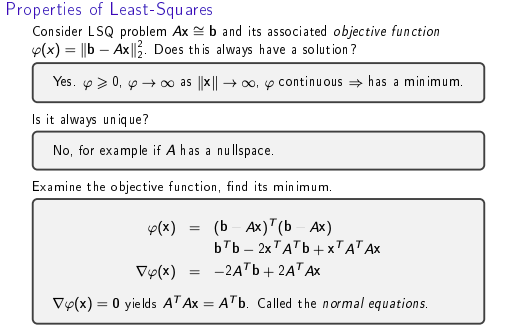
\includegraphics[width=\textwidth,height=\textheight,keepaspectratio]{lecture7_least_squares_prelim}
    \end{center}
    The textbook proves that there is always a unique vector $y \in \text{Span}(A)$ such that $\phi(y) = \norm{b - y}^2$ is minimal; as a consequence, there is at least one vector $x \in \R^m$ where $A$ is $\R^{n \times m}$ that minimizes $Ax \approx b$. This vector $x$ is unique iff $A$ is full rank.
\end{remark}

\begin{definition}
    A matrix $P$ is a projection if $P^2 = P$. A matrix is an orthogonal projection if $P^2 = P$ and $P^T = P$.
\end{definition}

\begin{proposition}
    If $P$ is an orthogonal projection, then the span of $P_{\perp} = (I - P)$ is orthogonal to the span of $P$.
\end{proposition}
\begin{proof}
    Given $x,y \in \R^n$, we see that

    \begin{align*}
        \inner{Px, (I - P)y} \\
        = \inner{Px, y - Py} \\
        = \inner{Px, y} - \inner{Px, Py} \\
        = \inner{Px, y} - \inner{x, Py} \\
        = 0
    \end{align*}
\end{proof}

\begin{corollary}
    Given an orthogonal projection $P$, any vector $x$ can be expressed as $x = Px + P_{\perp}x$.
\end{corollary}

\begin{proposition}
    The vector $x$ satisfying $\min_{x \in \R^n} \norm{Ax - b}_2$ is precisely the $x$ such that $Ax = Pb$ where $P$ is a projection onto $A$.
\end{proposition}

\begin{proof}
    Note that in what follows, all norms refer to the $2$ norm.
    \begin{align*}
        \norm{Ax - b} = \norm{P(Ax -b) + P_{\perp}(Ax - b)} \\
        \intertext{Since $P$ and $P_{\perp}$ map to orthogonal subspaces, we can apply the Pythagorean theorem} \\
        = \norm{P(Ax -b)} + \norm{P_{\perp}(Ax - b)} \\
        = \norm{P(Ax -b)} + \norm{-P_{\perp}b} \\
        = \norm{P(Ax -b)} + \norm{P_{\perp}b} \\
        = \norm{(Ax - Pb)} + \norm{P_{\perp}b} \\
        \intertext{The RHS is fixed, so we can only minimize the LHS} \\
    \end{align*}
\end{proof}

\begin{corollary}
    The $x$ aforementioned is $\inv{(A^TA)}A^Tb$ 
\end{corollary}
\begin{proof}
    \begin{align*}
        Ax = Pb \\
        \iff A^TAx = A^TPb \\
        \iff A^TAx = (PA)^Tb \\
        \iff A^TAx = (A)^Tb \\
        \iff x = \inv{(A^TA)}(A)^Tb \\
    \end{align*}
\end{proof}

\begin{proposition}
    $P = \inv{(A^TA)}A^T$ is an orthogonal projection, assuming
    that $A$ has full column rank.
\end{proposition}
\begin{proof}
    Verify to yourself that it is symmetric and $P^2 = P$. Also verify that $\text{span}(P) = \text{span}(A)$.
\end{proof}

\begin{corollary}
    The $x$ aformentioned is orthogonal to $b- Ax$, the residual.
\end{corollary}

\begin{proof}
    \begin{align*}
        b = Pb + P_{\perp}b \\
        \intertext{Substitute the definition of $x$ and $P$ found above}  \\
        b = Ax + (b - Ax) \\
    \end{align*}
\end{proof}

\begin{proposition}
    Suppose we know that the columns of $Q \in \R^{m \times n}$ form an orthonormal basis for $\text{span}(A)$. Then $QQ^T$ is an orthogonal projector for $A$.
\end{proposition}
\begin{proof}
    $(QQ^T)(QQ^T) = QQ^T$. Thus, this matrix is a projection; is it also clearly symmetric; finally, note that its span is precisely the span of $A$.
\end{proof}

\begin{corollary}
    With $Q$ as above and $P = QQ^T$, then the optimal $x$ satisfying $Ax \approx b$ is $Ax = Pb$. Leftmulitply both sides by $Q^T$ to obtain

    \[
        Q^TAx = Q^Tb
    \]

    If we do this, we can avoid the hassle of using the normal equations.
\end{corollary}

\begin{definition}
    I take the following as definitions. No time to look into their proofs:
    \begin{center}
        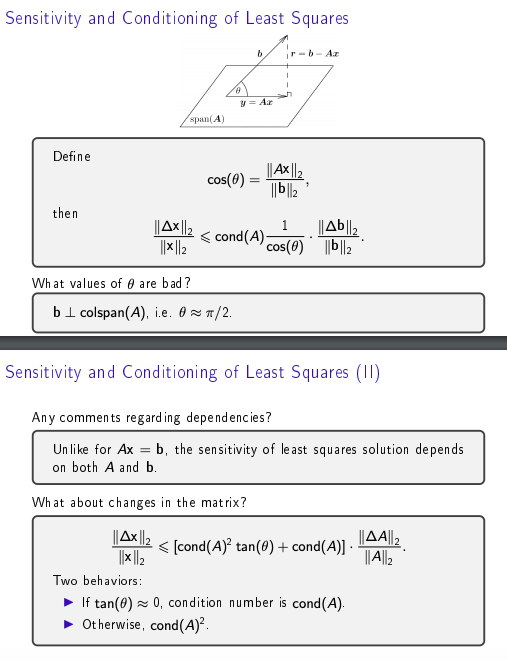
\includegraphics[width=\textwidth,height=\textheight,keepaspectratio]{lecture7_least_squares_cond}
    \end{center}
\end{definition}


\section{Lecture 8}{Problem Transformations}

\subsection{Quiz}
\begin{remark}
    If $Q$ is orthogonal, then $\norm{v} = \norm{Qv}$.
\end{remark}

\subsection{Householder Transformations}


\begin{remark}
    Recall that a matrix is orthogonal iff its transpose is its inverse.
    This means that both the rows and columns of the matrix, say $Q$, constitute an orthonormal set: the vectors are pairwise orthonormal, and they each have unit length.
\end{remark}
\begin{definition}
    
\end{definition}

\section{Lecture 9}{Problem Transformations II}

\section{Lecture 10}{SVD}

\begin{definition}
    Every matrix admits a decomposition:

    \[
        A = U \Sigma V^T
    \]

    The reduced SVD is the same decompositon but $\Sigma$ is reduced
    to be the small as possible.

    Entries of $U$ are called left singular vectors, entries in $\Sigma$ are singular values. Entries in $V^T$ can
\end{definition}

\begin{theorem}
    If $\norm{A} = \norm{\Sigma} = \sigma_1$ where $\sigma_1$ is the largest diagonal entry in $\Sigma$.
\end{theorem}

\begin{remark}
    If a singular value appearing in $\Sigma$ is negative, can it be made positive?
\end{remark}
\begin{solution}
    Yes, flip an appropriate singular vector in sign. UNRESOLVED.
\end{solution}

\begin{proposition}
    Take it for granted that $\norm{A}_2 = \sigma_1$. Given this, $k(A) = \frac{\sigma_1}{\sigma_{\min{m,n}}}$
\end{proposition}

\begin{proof}
    The inverse matrix will have all singular values of $A$ reciprocated.
\end{proof}

\begin{proposition}
   The null space of $V^T$ is given by the rows of $V^T$ corresponding to the singular values of $A$ (ie the values in $\Sigma$) that are $0$.
\end{proposition}
\begin{proof}
    Let these rows be collected in the set $V$. We argue
    that $V \s \mc{N}(A)$. Just hit $A$ by each $v_i \in V$.
\end{proof}

\begin{proposition}
    The rank of $A$ is given by the number of singular values
    that are not zero.
\end{proposition}
\begin{proof}
    $U$ and $V^T$ are full rank, so they cannot cause the rank to change. Only $\Sigma$ can.
\end{proof}

\begin{remark}
    Rank is not robust to rounding error. Suppose we have a rank one matrix; then introduce rounding error (each entry in the matrix has $\e_{mach}$ added or subtracted from it. By doing this, it is conceivable that the rank of the matrix is changed significantly. Far better, as a consequence, is to compute the numerical rank, which asks how many singular values fall above a tolerance. That is, for $\sigma \in \Sigma$, determine whether $\abs{\sigma} > \e$.
\end{remark}

\begin{theorem}{Eckhart Young Mirsky}
   The best $k$ rank approximation to $A$ is given by
   \[
       A_k = \sum_{i=1}^{k}\sigma_{i}u_{i}v_{i}^T
   \]
\end{theorem}
\begin{remark}
       Convince yourself that the summation above is the matrix
       that one obtains by, alternatively, zeroing all but the first
       $k$ diagonal entries of $\Sigma$ and then multiplying out
       $U \Sigma V^T$.
\end{remark}

\begin{remark}
    Using a $k$ rank approximation is not unambiguously good, for computation of the SVD requires $O(n^3)$ time.
\end{remark}

\begin{unresolved}
    If $A_k$ is the best $k$ rank approximation to $A$, is it the case that

    \[
        \norm{A_k - A}
    \]

    is the norm of the matrix obtained by zeroing out the first $k$ singular values of $A$.
\end{unresolved}

\begin{theorem}
    
\end{theorem}
\begin{proof}
    \begin{align*}
        U \Sigma V^T x \cong b \\
        \Sigma (V^Tx) \cong U^T b\\
        \Sigma y \cong U^T b \\
        \intertext{Solve for $y$} \\
        y_i = (U^Tb)_i/\sigma_i \text{ for } i\in [k]\\
        y_i = 0 \text{ ow }\\
    \end{align*}

    Then solve for $x$ where $V^Tx = y$. Note that $y$ is the optimal of all vectors $\hat{y}$ that solve $\Sigma \hat{y} \cong U^Tb$. It follows that $x$ is the minimal of all vectors that solve $Ax \cong b$ since $x = Vy$, meaning that $\norm{x}_2 = \norm{y}_2$.
\end{proof}

\begin{definition}
    The solution to the total least squares problem

    is $V \Sigma^{+} U^T b$ where $\Sigma^{+}$ is computed by reciprocating singular values in their spots (save those singular values that are $0$.
\end{definition}

\begin{remark}
    Remember the cost of householder for nonsquare
    and perhaps the cost for all $n \times n$ matrix.
\end{remark}

\end{document}










